% !TeX root = ../Thesis.tex

\chapter{Ergebnisse} \label{ch:results}


\section{Überblick}
Das nachfolgende Kapitel beschreibt die Ergebnisse der durchgeführten Experimente.
Die Experimente werden in mehreren Durchläufen der neu entwickelten 3D-Zelldaten-\linebreak Pipeline zur Auswertung von 3D-Zelldaten durchgeführt.
Auf Grundlage der Messergebnisse der 3D-Zelldaten-Pipeline wird eine statistische Auswertung durchgeführt. 
Zuerst werden die Bewertungen der Instanzsegmentierungsmasken anhand der \ac{ipq}-Metrik und anschließend die der Klassifikatoren anhand ihrer Genauigkeit betrachtet.\\[0.5\baselineskip]
Die \ac{ipq}-Ergebnisse werden in die drei Faktoren: \acf{sq}, \acf{rq} und die neu eingeführte \acf{iq} gegliedert (siehe Abschnitt \ref{sec:Kriterien}).
Daraus wird ersichtlich, dass jedes der Segmentierungsmodelle in einem der Faktoren dominiert, insgesamt aber CellposeSAM den anderen Modellen signifikant überlegen ist. 
Auch die Ergebnisse der Klassifikation werden unterteilt, um den Einfluss einzelner Methoden auf die Genauigkeit des Klassifikators zu identifizieren.
Vergleiche der Ergebnisse verschiedener Methoden zeigen, dass die neu eingeführten Methoden wie der Pseudo-Labler (siehe Abschnitt \ref{sec:Pretrain}) je nach Anforderung dem Stand der Technik entsprechen.
Außerdem zeigen die Ergebnisse, dass die Anwendung der 3D-Zelldaten-Pipeline optimale Methoden für die Segmentierung und Klassifikation von Zelldaten effizient ermittelt und gegenüber nicht-optimalen Methoden einen signifikanten Qualitätsunterschied aufweist.
Mithilfe ausführlicher Analysen lassen sich des Weiteren grundlegende Erkenntnisse über das Verhalten von Klassifikatoren im Umgang mit biologischen 3D-Bildstapeln gewinnen.

\section{Hardware}
Für die Anwendung wird eine NVIDIA GeForce RTX 3090 Ti mit 24 GB VRAM verwendet.
Der verwendete Server verfügt über eine 12th-Gen-Intel(R) Core(TM) i9-12900KF-CPU mit 16 Kernen und 64 GB RAM.

\section{Segmentierung}
Für die Wahl eines Segmentierungsmodells wird in Abschnitt \ref{sec:Kriterien} das Bewertungskriterium \ac{ipq} eingeführt.
Außerdem wird in Abschnitt \ref{sec:bench} der annotierte S\_BIAD1518-Datensatz vorgestellt.
Die \ac{ipq} wird auf dem Datensatz mit den Masken der drei vortrainierten Segmentierungsmodelle und zur Validierung anhand der Annotationen durchgeführt.
Alle Annotationen erreichen einen \ac{ipq}-Wert von genau Eins.
Abb. \ref{fig:example_masks} zeigt exemplarisch einen 2D-Schnitt eines 3D-Bildes mit roten Linien als Konturen der Annotation bzw. der vorhergesagten Segmentierungsmaske je Modell.
Die prädizierten Instanzsegmentierungsmasken für die dreidimensionalen Benchmarkdaten der drei Segmentierungsmodelle unterscheiden sich optisch deutlich (siehe Abb. \ref{fig:example_masks}).
Masken des nnUNet-Modells sehen kantiger aus als die Masken anderer Modelle und weisen oft eine raue Kontur mit hervorstehenden Extremitäten oder Einkerbungen auf.
Deepcell-Masken sehen glatt und ausgebreitet aus.
Durch die Watershed-Nachverarbeitung sind teilweise sichtbare Artefakte entstanden, an Stellen, an denen das Trennen der Instanzen für Watershed nicht möglich ist.
Die CellposeSAM-Masken sehen intuitiv am besten aus, sie haben oft nahezu eliptische Konturen und trennen Instanzen so wie es für das menschliche Auge sinnvoll erscheint. 
Das spiegelt sich auch in deutlichen Unterschieden in der \ac{ipq} wider.
\begin{figure}[H]
    \centering
    \begin{subfigure}[t]{0.24\textwidth}
        \includegraphics[width=\linewidth]{Figures/Deepcell_Mask_Example.png}
        \caption{Deepcell Maske.}
        \label{fig:DeepcellMaske}
    \end{subfigure}
    \hfill
    \begin{subfigure}[t]{0.24\textwidth}
        \includegraphics[width=\linewidth]{Figures/nnUNet_Mask_Example.png}
        \caption{nnUNet Maske.}
        \label{fig:nnUNetMaske}
    \end{subfigure}
    \hfill
    \begin{subfigure}[t]{0.24\textwidth}
        \includegraphics[width=\linewidth]{Figures/CellposeSam_Mask_Example.png}
        \caption{CellposeSam Maske.}
        \label{fig:CellposeSamMaske}
    \end{subfigure}
    \hfill
    \begin{subfigure}[t]{0.24\textwidth}
        \includegraphics[width=\linewidth]{Figures/gt_Mask_Example.png}
        \caption{Maske der Annotation.}
        \label{fig:gtMaske}
    \end{subfigure}
    \caption{Darstellung der Segmentierungsmasken der verschiedenen Segmentierungsmodelle sowie der Annotation als Konturen auf einem zweidimensionalen Durchschnitt einer dreidimensionalen Stichprobe des S\_BIAD1518-Datensatzes.}
    \label{fig:example_masks}
\end{figure}
\noindent
Die Ergebnisse jedes Segmentierungsmodells sind einzeln und für jedes Bild im Anhang \ref{supp:ipq} angehängt. 
Eine Zusammenfassung der \ac{ipq}-Ergebnisse ist in den Boxplots in Abb. \ref{fig:boxplots_ipq} gegeben.
Das zentrale Ergebnis ist, dass CellposeSAM die besten \ac{ipq}-Werte liefert. 
Mit einem Mittelwert von \num{0.64} liegt die \ac{ipq} von CellposeSAM über dem Mittelwert bei nnUNet (\num{0.04}) und Deepcell (\num{0.02}), wie höchst signifikante einseitige t-Tests zeigen. 
Dennoch zeigt sich, dass CellposeSAM lediglich in der Kategorie \ac{sq} den höchsten Mittelwert aufweist. 
Die \ac{rq} der nnUNet-Masken ist höher als die der CellposeSAM-Masken. 
Ebenso ist die \ac{iq} der Deepcell-Masken höher als die \ac{iq} der CellposeSAM-Masken.
Beide Beobachtungen sind durch höchst signifikante t-Tests gestützt. \\[0.5\baselineskip]
Obwohl nnUNet und Deepcell jeweils eine Metrik dominieren, wird ihr \ac{ipq}-Wert durch die beiden niedrigsten Faktoren stark heruntergezogen, während CellposeSAM in jeder Metrik gut, wenn auch nicht am besten, abschneidet.
Außerdem zeigen die Boxplots viele Ausreißer in den Daten, was den Unterschieden zwischen den Bildkategorien, die im Datensatz enthalten sind, geschuldet sein kann.
\begin{figure}[H]
    \centering
    \includegraphics[width=0.8\linewidth]{Figures/Segmentation_Boxplots.pdf}
    \caption{Ergebnisse der \ac{ipq}-Berechnungen mit den Faktoren $k_i = 1$ (siehe Formel (\ref{eq:ipq})). 
    Die X-Achse unterteilt die Daten in die Kriterien \acf{sq}, \acf{rq}, \acf{iq} und \acf{ipq}, wie in der Formel (\ref{eq:ipq}) beschrieben. 
    Für jede Metrik sind drei farbige Boxplots zu sehen, jeweils einer pro Segmentierungsmodell.
    Die Sterne zeigen die Signifikanz relevanter t-Tests an.
    }
    \label{fig:boxplots_ipq}
\end{figure}
\noindent
In Abb. \ref{fig:ipq_examples} sind Beispiele für die einzelnen Fehlerarten zu sehen.
Das \ac{iq}-Beispiel zeigt die Verletzung injektiver Abbildung der Nuclei auf die Annotation anhand einer nnUNet-Maske.
Zentral ist hier ein nicht eliptischer Nucleus zu sehen.
\newline\begin{figure}[H]
    \centering
    \includegraphics[width=0.65\linewidth]{Figures/IPQ_examples.pdf}
    \caption{Exemplische Darstellung einzelner Ausprägungen verschiedener Fehlerarten.
    Hierzu sind jeweils, in dieser Reihenfolge von links nach rechts, ein Ausschnitt eines 2D-Durchschnitts einer Stichprobe, die Annotation als Kontur und die vorhergesagte Maske eines Modells zu sehen.
    Die erste Zeile zeigt ein Beispiel für einen schlechten \ac{iq}-Wert anhand einer nnUNet-Maske.
    In der zweiten Zeile ist ein \ac{rq}-Fehler anhand einer CellposeSAM-Maske zu sehen und unten ist ein Beispiel für einen schlechten \ac{sq}-Wert anhand einer Deepcell-Maske zu sehen. 
    }
    \label{fig:ipq_examples}
\end{figure}
\noindent
Dieser Nucleus wird vom nnUNet-Modell in mehrere Segmente unterteilt, wodurch die räumliche Konzentration der Nuclei überschätzt wird.
Nicht-eliptische Nuclei führen häufig zu dieser Art von Fehlern.\\[0.5\baselineskip]
Mit dem Fehler gehen \ac{rq}-Fehler einher, weil zwei der Segmente im Vergleich zur Annotation zu klein sind, um als \ac{tp} erkannt zu werden.
In der zweiten Zeile ist anhand einer CellposeSAM-Maske ein \ac{rq}-Beispiel dargestellt.
Das Segmentierungsmodell hat hier einen Nucleus halluziniert. 
Der Nucleus unten links, direkt unter dem Linken der beiden großen Nuclei, ist in der Annotation nicht zu finden.
Dieser Fehler geht nicht mit einem schlechteren \ac{sq}- oder \ac{iq}-Wert einher.
Durch den Fehler wird die Anzahl der Nuclei überschätzt.\\[0.5\baselineskip]
Zuletzt ist ein \ac{sq}-Beispiel dargestellt.
Neben und unter dem sichtbaren Nucleus oben sind vermutlich Schatten von Nuclei aus anderen Z-Ebenen zu sehen, die vom Deepcell-Modell als Nuclei erfasst wurden.
Dadurch ist das Segment, das den sichtbaren Nucleus abbildet, deutlich zu groß, was die \ac{iou}-Werte beeinträchtigt.
Mit diesem Fehler geht auch ein schlechterer \ac{rq}-Wert einher, da der Schatten zu mehreren Halluzinationen geführt hat.
Da diese Halluzinationen nicht mit den Annotationssegmenten überschneiden, ist der \ac{iq}-Wert hier nicht betroffen.
Der Fehler führt zu einer Fehleinschätzung des Nucleivolumens.\\[0.5\baselineskip]
Abb. \ref{fig:contour_examples} zeigt ein Beispiel für eine Instanzsegmentierungsmaske der Zieldaten mit dem CellposeSAM-Modell.
\begin{figure}[H]
    \centering
    \includegraphics[width=0.98\linewidth]{Figures/contour_examples.pdf}
    \caption{Exemplische Darstellung einer Zieldaten-Instanzsegmentierungsmaske des CellposeSAM-Modells.
    Links ist eine 2D-Schicht des Original-Bildes zu sehen, daneben die Instanzsegmentierungsmaske und rechts eine Überlagerung von den Konturen der Instanzen über die Marker-Kanäle des Originals. 
    Zu jeder der drei Ansichten sind auch 2D-Schnitte der X-Z-Ebene und der Y-Z-Ebene gegeben.
    }
    \label{fig:contour_examples}
\end{figure}
\noindent
Links sind exemplarisch 2D-Schichten eines 3D-Eingabevolumens zu sehen.
Die Schichten sind Schnitte durch die drei Koordinaten-Ebenen des Volumens.
Daneben ist die Instanzsegmentierungsmaske als Maskenbild und als Konturen auf den Marker-Kanälen des Eingabebilds dargestellt.
Zu sehen ist, dass die CellposeSAM-Masken auch intuitiv sehr gut zur Eingabe passen.
\section{Klassifikation}\label{sec:resultsClassifier}
\subsection{Überblick}
Die in Abschnitt \ref{sec:MethodsClassifier} eingeführten Methoden zur Klassifikation werden anhand eines separaten Anteils des manuell annotierten Datensatzes durch die neu entwickelte 3D-Zelldaten-Pipeline getestet.
Der manuell annotierte Datensatz enthält 125 Stichproben von \linebreak Myotuben-Zellkernen, 95 Stichproben der Klasse Debris, 148 Stichproben der Klasse \glqq Andere\grqq und nur 16 Stichproben der Klasse Schwannzellen-Nucleus.
Die Klassen Eins bis Vier sind hier der Reihe nach Myotuben-Kerne, Debris, \glqq Andere\grqq und Schwannzellen-Kerne.
Der Abschnitt \ref{supp:Klassifikation} des Anhangs zeigt alle Ergebnisse der verschiedenen Methodenkombinationen tabellarisch.
Um die Genauigkeit der Klassifikatoren anhand des Test-Anteils möglichst repräsentativ zu bestimmen, werden manuell 50\% statt 20\% der Schwannzellen-Nuclei in den Test-Anteil der Daten eingesetzt.
Die Genauigkeit, also der prozentuale Anteil richtiger Vorhersagen, auf dem Test-Anteil des Zieldatensatzes wird als Kriterium verwendet.\\[0.5\baselineskip]
Da die Modelle während des Trainings rauschbehaftete Verläufe der Genauigkeit aufweisen und es zu Overfitting kommen kann, wird Early-Stopping implementiert, wobei die mittlere Genauigkeit des Klassifikators auf dem Test-Anteil der manuell annotierten Daten über fünf Epochen hinweg gemessen wird.
Dazu wird die geglättete Genauigkeit berücksichtigt.
Wenn diese viermal in Folge sinkt oder gleich bleibt, wird das Training unterbrochen.
Abb. \ref{fig:Trainingsverlauf} zeigt exemplarisch zwei Trainingsverläufe, die dieses Phänomen belegen.
\begin{figure}[H]
    \centering
    \includegraphics[width=0.98\linewidth]{Figures/Trainingskurven.pdf}
    \caption{Die Diagramme zeigen den Trainingsverlauf eines Klassifikators. 
    Links ist der Verlauf des Loss zu sehen.
    In der Mitte und rechts sind die Verläufe der Validierungsgenauigkeit zu sehen.
    Rechts ist die Kurve zur Anschaulichkeit durch Mittelung von je fünf Werten geglättet.
    Der obere Verlauf zeigt einen Klassifikator ohne Overfitting, im unteren Verlauf ist Overfitting zu erkennen.
    }
    \label{fig:Trainingsverlauf}
\end{figure}
\noindent
Im oberen Verlauf ist zu sehen, dass die Genauigkeit des Klassifikators tendenziell steigt.
Die geglättete Genauigkeit zeigt hier zwar rauschbehaftetes Verhalten mit einigen lokalen Minima, aber nach ein bis zwei Berechnungsschritten steigt der Wert wieder.
Der Verlauf ist zwar nicht monoton steigend, aber es liegt nahe, dass bei Fortsetzung des Trainings weitere Verbesserungen zu erwarten sind.
Im unteren Verlauf ist Overfitting zu erkennen, da die geglättete Genauigkeit über vier Berechnungsschritte hinweg gesunken oder gleich geblieben ist.
Der Trainings-Loss nimmt in den gleichen Epochen weiter ab.
Das Modell passt sich also weiter an die Trainingsdaten an, ohne dass es besser darin wird, ungesehene Nuclei zu erkennen.
Die Genauigkeit auf dem Test-Anteil des Datensatzes sinkt etwa ab Epoche 30 und erreicht ihr Maximum in Epoche 32. 
Dementsprechend wird die Genauigkeit des Klassifikators in Epoche 32 für den Vergleich herangezogen. %\\[0.5\baselineskip]
Mit der Prädiktion erweitern die Klassifikatoren die Instanzsegmentierungsmasken zu panoptischen Segmentierungsmasken.
Abb. \ref{fig:contours_classes} zeigt exemplarisch eine panoptische Maske.
\begin{figure}[H]
    \centering
    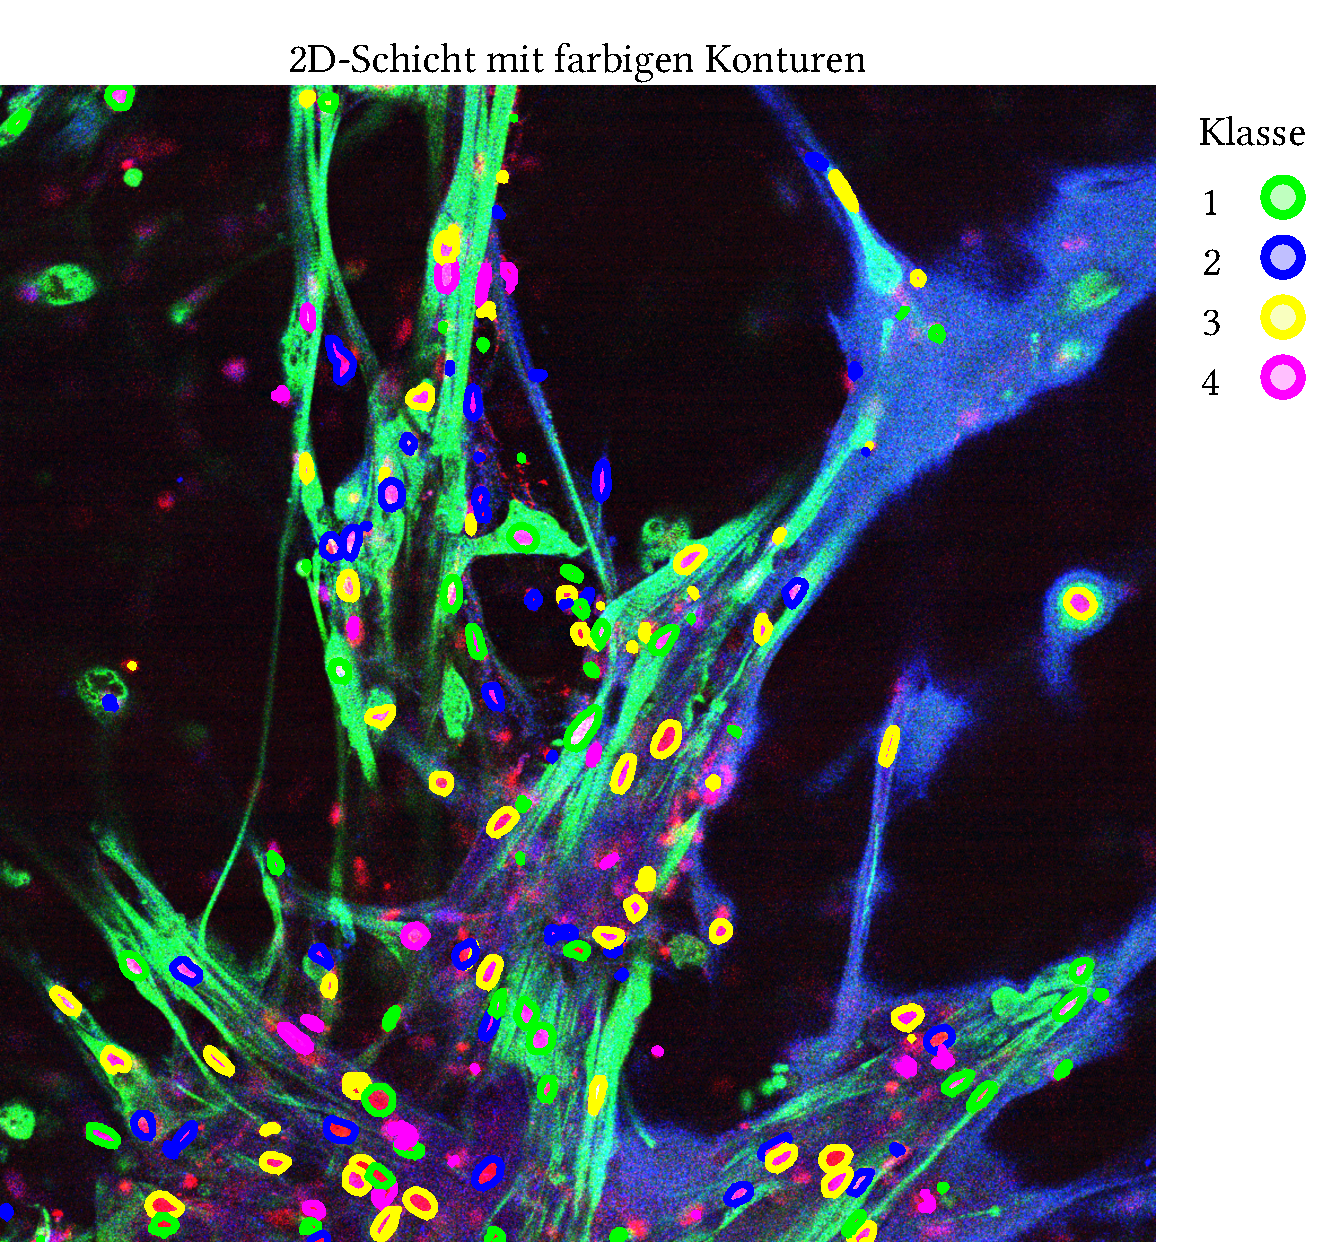
\includegraphics[width=0.98\linewidth]{Figures/contours_and_classes.pdf}
    \caption{Panoptische Segmentierungsmaske, erstellt durch die Kombination der Instanzsegmentierungsmaske des CellposeSAM-Segmentierungsmodells und der prädizierten Klassen eines Klassifikators.}
    \label{fig:contours_classes}
\end{figure}
\noindent
Die Klassen eins bis vier sind der Reihe nach Myotuben-Kerne, Debris, \glqq Andere\grqq und \linebreak Schwannzellen-Kerne.
Die Konturfarben der Nuclei kennzeichnen ihre Klassen.\\[0.5\baselineskip]
Ganz rechts in der Mitte der 2D-Schicht ist ein Beispiel für eine fehlklassifizierung zu sehen. 
Die Kontur ist gelb, was bedeutet, die Vorhersage ist die Klasse \glqq Andere\grqq.
Tatsächlich spricht aber die grüne Umgebung des Nucleus dafür, dass es sich um einen Myotuben-Zellkern handelt, der untypischerweise nicht elliptisch, sondern annähernd kreisförmig ist, weil die Muskelfaser orthogonal zur Bildebene verläuft.
\subsection{Encoder}\label{subsec:RES_encoder}
In Abb. \ref{fig:bars_encoders} ist die Genauigkeit der Klassifikatoren pro Encoder gegeben.
Zu sehen ist sowohl das Maximum, als auch der Durchschnitt der Genauigkeitswerte der verschiedenen Methodenkombinationen jedes Klassifikators.
Die Klassifikatoren sind nach dem aufsteigenden Maximalwert sortiert.
\begin{figure}[H]
    \centering\includegraphics[width=0.8\linewidth]{Figures/encoders_compare.pdf}
    \caption{Das Balkendiagramm zeigt an der Y-Achse die Genauigkeit der Klassifikatoren bei der Verwendung der verschiedenen Encoder.
    Auf der X-Achse sind die Encoder in Gruppen angeordnet.
    Jede Gruppe enthält einen Maximalwert (Orange) und einen Durchschnittswert (Blau), da jeder Encoder mit verschiedenen Kombinationen von Methoden getestet wird.
    Die Encoder sind nach aufsteigendem Maximalwert von links nach rechts sortiert.
    }
    \label{fig:bars_encoders}
\end{figure}
\noindent
Zu sehen ist, dass der beste Wert vom ResNet18-Encoder stammt.
Mit 85,9\% Genauigkeit auf dem Test-Anteil des Datensatzes ist diese Kombination das gefundene Optimum.
Auch im Mittelwert haben die Klassifikatoren mit dem ResNet18-Encoder mit 79,1\% die höchste Genauigkeit.
CellposeSAM und ResNet101 haben als Encoder die zweit- und dritthöchsten durchschnittlichen Genauigkeiten mit 77,4\% und 77,3\%, jeweils.
Während CellposeSAM allerdings die zweithöchste maximale Genauigkeit aufweist, hat ResNet101 die geringste.
Besonders auffällig ist Swin V2.
Mit 64,6\% hat es die niedrigste durchschnittliche Genauigkeit, aber der Maximalwert von 83,9\% ist der dritthöchste.
Besonders häufig werden mit beiden Klassifikations-Köpfen die Klassen Schwannzellen-Kern mit Myotuben-Kernen und die Klasse \glqq Andere\grqq mit Debris verwechselt.
Abb. \ref{fig:Decoder_errors} zeigt einige Beispiele dieser Verwechslung.
\begin{figure}[H]
    \centering
    \includegraphics[width=0.98\linewidth]{Figures/Slice_Decoder_1and4.pdf}
    \caption{Beispiele für die Verwechslung von Schwannzellen-Kernen und Myotuben-Kernen sowie \glqq Andere\grqq und Debris}
    \label{fig:Decoder_errors}
\end{figure}
\noindent
\subsection{Vortraining}\label{subsec:RES_pretrain}
Abb. \ref{fig:heatmap_pretrain} zeigt eine Übersicht über die Effektivität der verwendeten Vortrainingsmethoden.
\begin{figure}[H]
    \centering\includegraphics[width=0.7\linewidth]{Figures/encodersVpretrain.pdf}
    \caption{Die Heatmap zeigt die Genauigkeiten der Klassifikatoren bei der Verwendung der verschiedenen Vortrainingsmethoden.
    Auf der Y-Achse sind die verschiedenen Encoder aufgeführt.
    Die X-Achse zeigt die getesteten Methoden des Vortrainings an.
    Die Farbe der Felder und der Wert darin zeigen die Durchschnittsgenauigkeiten aller Klassifikatoren, die die jeweilige Vortrainingsmethode nutzen.
    Die letzte Zeile zeigt den Durchschnitt der Werte aller Encoder, abhängig von der Vortrainingsmethode.}
    \label{fig:heatmap_pretrain}
\end{figure}
\noindent
Um die Ergebnisse möglichst unabhängig von den anderen Klassifikatormethoden zu betrachten, werden hier nur die Klassifikatoren mit der besten Vorverarbeitungsmethode für den Encoder und dem Volumen-Klassifikator als Klassifikations-Kopf betrachtet.
Auf der vertikalen Achse sind die verschiedenen Encoder sowie der Durchschnitt aller Encoder zu sehen.
Auf der horizontalen Achse sind die vier Vortrainingsmethoden aufgeführt.
Links ist nur semi-supervised-Training zu sehen.
Daneben steht das semi-supervised-Vortraining, also das Vortraining mit den Pseudo-Labler-Annotationen, Einfrieren der \linebreak Encoder-Gewichte und Fortsetzen des Trainings mit vollständig annotierten Daten zu sehen. 
Rechts ist das fully-supervised ImageNet-Vortraining mit eingefrorenen Encoder-Gewichten und \glqq kein Vortraining\grqq aufgetragen (siehe Abschnitt \ref{sec:Pretrain}).\\[0.5\baselineskip]
Zu sehen ist, dass das Vortraining mit semi-supervised-Daten durchschnittlich deutlich schlechtere Ergebnisse liefert als das fully-supervised ImageNet-Vortraining und etwas schlechtere Ergebnisse als kein Vortraining.
Im Durchschnitt führt das Fortführen des Trainings mit den annotierten Daten nach dem semi-supervised-Vortraining zu einer Steigerung der Genauigkeit um 13 Prozentpunkte.
Für den ConvNeXt-Encoder ist der Vorteil des fortgesetzten Trainings besonders hoch mit 39 Prozentpunkten.
Der ConvNeXt-Encoder ist außerdem mit dem semi-supervised-Vortraining um sieben Prozentpunkte genauer als ohne Vortraining.
Auch die beiden ResNet-Modelle erzielen mit dem semi-supervised-Vortraining ähnlich gute Ergebnisse wie mit anderen Vortrainingsmethoden.
Im Vergleich zum ImageNet-Vortraining, das deutlich mehr Rechenaufwand erfordert, sind die Klassifikatoren mit ResNet18 und ResNet101 nur um zwei bzw. drei Prozentpunkte schlechter, wenn sie die Annotationen des Pseudo-Lablers als Vortraining nutzen.
Beide haben außerdem eine höhere Genauigkeit als der Durchschnitt ohne Vortraining.
Sie sind beide auch ohne Fortsetzung des Trainings nach dem semi-supervised-Vortraining bereits 64\% und 62\% genau. \\[0.5\baselineskip]
Besonders auffällig ist auch hier das Swin V2-Modell, das ohne \linebreak fully-supervised-Vortraining nur eine durchschnittliche Genauigkeit von 44,0\% erreicht.
Vortraining auf dem ImageNet-Datensatz führt im Vergleich dazu bei diesem Encoder zu einer Steigerung der Genauigkeit um 40 Prozentpunkte.
Wie in Abschnitt \ref{subsec:RES_encoder} beschrieben, hat die Genauigkeit des Swin V2-Encoders einen hohen Maximalwert, aber einen geringen Durchschnittswert.
Der Vergleich der Vortrainingsmethoden zeigt, dass das an der schlechten Leistung des Swin V2-Encoders ohne ImageNet-Vortraining liegt.\\[0.5\baselineskip]
Abb. \ref{fig:gradCAM_Swin} zeigt zwei Scatterplots.
Beide visualisieren Projektionen des Merkmalsraums des Swin V2-Ecoders in zwei Dimensionen mittels \ac{tsne}.
Die linke Abbildung zeigt den Merkmalsraum des Encoders ohne Vortraining und die rechte den Merkmalsraum nach ImageNet-Vortraining.
Zu sehen ist, dass der Swin V2-Encoder keinen sinnvollen Merkmalsraum erlernt.
Das Vortraining auf dem ImageNet-Datensatz ist umfangreicher und diverser als auf den Zieldaten und führt dadurch zu einem generalisierteren Merkmalsraum.
ImageNet-Vortraining liefert im Durchschnitt die besten Ergebnisse mit einer Genauigkeit von 84\%. 
Außerdem ist die Varianz entlang der Encoder mit dem ImageNet-Vortraining (\num{5.6e-5}) deutlich geringer als ohne Vortraining (0,016). 
Dennoch erreicht ResNet18 ohne Vortraining die beste Genauigkeit mit 86\%. 
\newpage
\begin{figure}[H]
    \centering
    \begin{subfigure}[t]{0.49\textwidth}
        \includegraphics[width=\linewidth]{Figures/swin_bad.pdf}
    \end{subfigure}
    \hfill
    \begin{subfigure}[t]{0.49\textwidth}
        \includegraphics[width=\linewidth]{Figures/swin_good.pdf}
    \end{subfigure}
    \caption{2D-Projektionen des Merkmalraums zweier Klassifikatoren mittels \ac{tsne}.
    Der linke Scatterplot zeigt den Merkmalsraum eines Swin V2-Encoders ohne Vortraining, der rechte den eines ImageNet-vortrainierten Swin V2-Encoders.}
    \label{fig:gradCAM_Swin}
\end{figure}
\noindent
Des Weiteren wird die durchschnittliche Genauigkeit pro Klasse betrachtet.
Abb. \ref{fig:per_class_acc} zeigt die durchschnittliche Genauigkeit pro Klasse und Sterne als Hinweise auf signifikante Ergebnisse von paarweisen t-Tests.
In jedem Balken des Diagramms ist je ein Beispiel der Klassen ohne Vorverarbeitung als 2D-Schnitt gegeben. 
In Rot sind die Nucleus-Kanäle dargestellt, Grün und Blau sind Marker-Kanäle.
Die Nuclei der Klasse Myotuben-Kern Schwannzellen-Kern sind optisch sehr ähnlich, beide sind lang und dünn.
Die Unterscheidung ist nur durch die Betrachtung der umliegenden Strukturen möglich.\\[0.5\baselineskip] 
Wie eingangs beschrieben, sind im Datensatz nur 16 Beispiele der Klasse Schwannzellen-Nucleus enthalten, davon acht im Trainings- und acht im Test-Anteil.
Zu sehen ist, dass insbesondere die Schwannzellen-Kerne schlecht erkannt werden.
Wie in Abschnitt \ref{sec:Preproc} beschrieben, wird dieses Problem der ungleichen Verteilung der Klassen mithilfe des Retreivers durch eine Gewichtung der Gradienten unterrepräsentierter Klassen angegangen.
In der Abbildung ist jedoch zu sehen, dass dieser Ansatz das Problem nicht vollständig löst. 
Die unterrepräsentierte Klasse der Schwannzellen-Nuclei wird dennoch schlechter erkannt als alle anderen Klassen.
Beinahe alle Methoden ergeben isoliert betrachtet eine ähnliche Verteilung der Genauigkeit pro Klassen, nur das Vortraining hat einen Einfluss.
Vortraining mit semi-supervised-Annotationen und anschließendes Fortsetzen des Trainings mit manuell annotierten Daten führen zu Klassifikatoren, die teilweise wesentlich ausgeglichener die Klassen erkennen.
Mit dem Volumen-Klassifikator und der Masken-Methode zur Vorverarbeitung erreichen der ResNet101-Encoder 83,2\%, der ResNet18-Encoder 73,5\% und der  ConvNeXt-Encoder 56,3\% Genauigkeit für die Klasse der Schwannzellen-Nuclei.
Die durchschnittliche Genauigkeit für die Schwannzellen-Klasse mit diesen Methodenkombinationen beträgt 71\%.
Das ist im Vergleich zu den 21,7\% durchschnittlicher Genauigkeit für die Schwannzellen-Klasse ein starker Genauigkeitszuwachs. 
Die durchschnittliche Genauigkeit ist nach dem semi-supervised-Vortraining also geringer, aber dafür wird die unterrepräsentierte Klasse der Schwannzellen-Kerne nicht, wie bei anderen Vortrainingsmethoden, schlechter erkannt.
\begin{figure}[H]
    \centering
    \includegraphics[width=0.98\linewidth]{Figures/per_class_acc.pdf}
    \caption{Durchschnittliche Genauigkeit pro Klasse aller Klassifikatoren.
    Die Klassen sind Myotuben-Kerne, Debris, \glqq Andere\grqq und Schwannzellen-Kerne.
    Unten in den Balken ist je ein Beispiel für die entsprechende Klasse als 2D-Schnitt gegeben.
    }
    \label{fig:per_class_acc}
\end{figure}
\noindent 
\subsection{Klassifikations-Kopf}\label{subsec:RES_decoder}
Abb. \ref{fig:bars_decoders} zeigt eine Gegenüberstellung der Genauigkeit beider Klassifikations-Köpfe in einem Balkendiagramm mit Fehlerbalken.
\begin{figure}[h!]
    \centering\includegraphics[width=0.78\linewidth]{Figures/encodersVdecoder.pdf}
    \caption{Genauigkeitswert der Klassifikatoren unter Verwendung eines bestimmten Klassifikations-Kopfes.
    Auf der Y-Achse ist der Durchschnitt der Genauigkeiten der besten Trainingsepoche aller Klassifikatoren, die diesen Klassifikations-Kopf nutzen, aufgetragen. 
    Die X-Achse zeigt Gruppen von Encodern, jeweils besetzt mit einem Wert für den Schichten- und den Volumen-Klassifikator.
    Rechts zu sehen sind Balken, die den Durchschnitt der Werte aller Encoder, abhängig von dem Klassifikations-Kopf, zeigen.}
    \label{fig:bars_decoders}
\end{figure}
\noindent
Dabei werden nur die Klassifikatoren berücksichtigt, bei denen sich die Methodenkombination ausschließlich im verwendeten \linebreak Klassifikations-Kopf unterscheidet.
Das ist notwendig, da nicht alle möglichen Kombinationen trainiert wurden und ein Vergleich mit unvollständigen Kombinationen keine aussagekräftigen Ergebnisse liefert.  
Die blauen Balken des Balkendiagramms zeigen jeweils die Ergebnisse der Architekturen, die den Schichten-Klassifikator nutzen, die orangenen Balken die Ergebnisse des Volumen-Klassifikators.
Auf der X-Achse sind als Gruppen zuerst die Encoder und zuletzt der Durchschnitt aufgetragen, und auf der Y-Achse die durchschnittliche Genauigkeit der Modelle mit dem jeweiligen Klassifikations-Kopf.
An den Daten lässt sich erkennen, dass der Einfluss des Klassifikations-Kopfes nicht homogen ist.
Mit dem ConvNeXt-Encoder ist der Schichten-Klassifikator performanter als der Volumen-Klassifikator, während es bei allen anderen Encodern umgekehrt ist.
Für den CellposeSAM Encoder ist der Genauigkeitsunterschied 12,6 Prozentpunkte groß, für EfficientNetV2 einen halben Prozentpunkt.\newline%\\[0.5\baselineskip]
Die Daten zeigen also, dass die Intensität des Unterschieds in der Genauigkeit der beiden Klassifikations-Köpfe stark vom Encoder abhängt.
Die Balken rechts, die je den Durchschnitt aller Modelle mit einem Klassifikations-Kopf darstellen, zeigen signifikant, dass der Volumen-Klassifikator bessere Ergebnisse liefert.\\[0.5\baselineskip]
Mit dem Schichten-Klassifikator werden häufig Nuclei fehlerhaft klassifiziert, die nicht in der mittleren Schicht des Bildausschnitts vorkommen.
Die Nuclei sind oft in den obersten Schichten der Eingabedaten zu finden.
Wenn sie nicht mindestens zwölf Ebenen von der obersten Z-Ebene entfernt sind, schneidet der Retreiver Bildausschnitte aus, in denen die Nuclei in Z-Richtung nicht zentriert sind.
Abb. \ref{fig:Sclice_decoder_slices} zeigt fünf Ebenen eines Nucleus, für die das zutrifft.
\begin{figure}[H]
    \centering
    \includegraphics[width=0.98\linewidth]{Figures/Slice_Decoder_Ebenen.pdf}
    \caption{Fünf 2D-Schichten eines fehlklassifizierten Nucleus.
    Die Z-Ebene ist über den Abbildungen angegeben.
    Zu sehen ist, dass der Nucleus nicht zentriert ist und nicht in der mittleren Schicht präsent ist.}
    \label{fig:Sclice_decoder_slices}
\end{figure}
\noindent
Der Nucleus ist mit der Masken-Methode vorverarbeitet und in Rot zu sehen.
Er erscheint nicht in den Schichten zehn und zwölf.
Schicht acht zeigt gerade die untere Kante des Nucleus. 

\subsection{Vorverarbeitung}\label{subsec:RES_preproc}
In Abb. \ref{fig:bars_channel1} sind die durchschnittlichen Genauigkeiten der Modelle gezeigt, die jeweils eine der Vorverarbeitungsmethoden nutzen.
\begin{figure}[H]
    \centering\includegraphics[width=0.8\linewidth]{Figures/encodersVchannel1.pdf}
    \caption{Genauigkeitswert der Klassifikatoren bei Verwendung einer bestimmten Vorverarbeitungsart.
    Auf der Y-Achse ist der Durchschnitt der Genauigkeiten der besten Trainingsepoche aller Klassifikatoren, die diese Vorverarbeitungsart nutzen, aufgetragen. 
    Die X-Achse zeigt Gruppen von Encodern, jeweils besetzt mit einem Wert für die Masken-Methode, die den Nucleus-Kanal des Bildes durch die Segmentierungsmaske ersetzt, und die Distanz-Methode, die eine Distanztransformation auf den Nucleus-Kanal anwendet.
    Rechts zu sehen sind Balken, die den Durchschnitt der Werte aller Encoder, abhängig von der Vorverarbeitungsmethode, zeigen.}
    \label{fig:bars_channel1}
\end{figure}
\noindent
Wie für den Vergleich Klassifikations-Kopf-Architekturen sind auch hier die Klassifikatoren ausgeschlossen, deren Methodenkombination mit nur einer der beiden Vorverarbeitungsmethoden trainiert wurde.
Auf der Y-Achse ist die Genauigkeit aufgetragen, auf der X-Achse sind die Encoder und der Durchschnitt aller Encoder als Gruppen.
Die Ergebnisse zeigen deutlich, dass die Masken-Methode, also das Ersetzen des Nucleus-Kanals durch die Segmentierungsmaske, zu einer höheren Genauigkeit führt.
Mit der Distanz-Methode, also dem Anwenden einer Distanztransformation der Segmentierungsmaske auf den Nucleus-Kanal, beträgt die Genauigkeit durchschnittlich 77,2\%, mit der Masken-Methode sind es 81,5\%.
Die Differenz ist hoch signifikant.
Zu sehen ist aber, dass der Einfluss der Vorverarbeitung unterschiedlich stark ist, je nach Encoder.
Während die Genauigkeit für Modelle mit dem ResNet101-Encoder mit der Masken-Methode um 0,8 Prozentpunkte gegenüber der Distanz-Methode steigt, macht die Vorverarbeitung beim EfficientNet V2-Encoder 11,5 Prozentpunkte aus. \\[0.5\baselineskip]
Mit der Distanz-Methode treten häufig Fehler auf, wenn Nuclei dicht aneinander liegen.
Abb. \ref{fig:nuclei_overlap_examples} zeigt Nuclei mit der Distanz-Methode und der Masken-Methode, für die mit der Distanz-Methode eine schlechtere Genauigkeit erzielt wird als mit der Masken-Methode.
\begin{figure}[H]
    \centering\includegraphics[width=0.9\linewidth]{Figures/Cluster_MaskVDist.pdf}
    \caption{Beispiele für Nuclei, die häufig mit der Masken-Methode korrekt und mit der Distanz-Methode fehlerhaft klassifiziert werden.
    In der oberen Zeile sind die Nuclei zu sehen, die mit der Distanz-Methode vorverarbeitet sind.
    Darunter ist jeweils der gleiche Nucleus mit der Masken-Methode zu sehen.}
    \label{fig:nuclei_overlap_examples}
\end{figure}
\noindent
Die Nuclei in den Beispielen sind alle in Clustern angeordnet und berühren umliegende Nuclei.
Mit der Masken-Methode sind die umliegenden Nuclei ausgeblendet, mit der Distanz-Methode gehen sie in den betrachteten Nucleus über.
Intuitiv lassen sich die Nuclei auch mit der Distanz-Methode trennen, wie die Ergebnisse zeigen, ist das den Klassifikatoren aber nicht immer möglich.\\[0.5\baselineskip]
Mithilfe von Grad-CAM \cite{Selvaraju2017} wird außerdem das Verhalten der Klassifikatoren exemplarisch visualisiert.
Abb. \ref{fig:gradCAM} zeigt den Nucleus-Kanal und einen Marker-Kanal aus zwei 2D-Schichten.
\begin{figure}[h!]
    \raggedright
    \includegraphics[width=0.8\linewidth]{Figures/gradCAM.pdf}
    \caption{Grad-CAM-Visualisierung für zwei exemplarische 2D-Schichten, jeweils mit einem Nucleus-Kanal und einem Marker-Kanal.
    Links ist ein Beispiel einer Stichprobe gegeben, die mit der Masken-Methode trainiert wurde, rechts mit der Distanz-Methode.
    Die Nucleus-Kanäle zeigen die Segmentierungsmasken der Nuclei in Weiß, überlagert mit den gradientenbasierten Heatmaps, die die Wichtigkeit räumlicher Regionen für die Klassifikation darstellen.
    In beiden Nucleus-Kanälen ist die Wichtigkeit der Nucleus-Oberfläche nur sehr gering.
    In den Marker-Kanälen ist zu sehen, dass Regionen mit erkennbaren Strukturen besonders wichtig sind.}
    \label{fig:gradCAM}
\end{figure}
\noindent
Die beiden 2D-Schichten sind aus unterschiedlichen 3D-Stapeln, links einer, der mit der Masken-Methode, und rechts einer, der mit der Distanz-Methode vorverarbeitet wurde.
Zu sehen sind jeweils Heatmaps für zwei Klassifikatoren.
Beide Heatmaps zeigen gradientenbasiert die Aktivierungen in einer Schicht des Merkmalsraums auf die Eingangsdaten zurückprojiziert.
Die Heatmaps sind jeweils zur besseren Interpretierbarkeit einer 2D-Schicht der Segmentierungsmaske des Nucleus und eines Marker-Kanals überlagert. 
Dadurch wird räumlich aufgezeigt, welche Regionen der Eingangsdaten zur Entscheidung für eine bestimmte Klasse besonders beigetragen haben.
Die beiden Nucleus-Kanal-Ansichten zeigen, dass Regionen direkt um den Nucleus herum für die Klassifikationsentscheidung wichtiger sind als die Oberfläche des Nucleus.
Selbst unter Verwendung der \linebreak Distanz-Methode, die zum Ziel hat, Oberflächen-Merkmale zu erhalten und dafür klare Kanten und eine eindeutige Geometrie der Segmentierungsmaske augibt, wird die Oberfläche kaum betrachtet.
Des Weiteren sind in den Heatmaps der Marker-Kanäle zu sehen, dass auch abseits des Nucleus-Kanals eine intuitiv sinnvolle Lokalisierung der Aufmerksamkeit des Klassifikators erfolgt.
Die Maxima der Heatmaps sind auf sichtbare Strukturen im Marker-Kanal platziert.

\subsection{Wichtigkeit der Marker}\label{subsec:RES_allg}
Eine weitere angestellte Untersuchung ist die Quantifizierung der Wichtigkeiten der verschiedenen Marker-Kanäle. 
Auch für Expert*Innen ist es schwer, eindeutige Beziehungen zwischen den Strukturen, die durch bestimmte Marker gefärbt werden, und den verschiedenen Klassen der Nuclei herzustellen. 
Zur Abschätzung der globalen Markerrelevanz werden die Gradienten der Modellvorhersage bis auf die Eingangsebene zurückprojiziert und die betragsmäßigen Gradienten über die räumlichen Dimensionen gemittelt. 
Die Wichtigkeitswerte, die sich ergeben, sind nahezu gleich verteilt. \newline%, was darauf hindeutet, dass das Modell keine einzelnen Marker stark bevorzugt, sondern  kombinierte Informationen mehrerer Kanäle nutzt, um Entscheidungen zu treffen.
Abb. \ref{fig:marker_gradCAM} zeigt exemplarisch Gradientenfelder einer 2D-Schicht aus einer Stichprobe der dreidimensionalen Zieldaten sowie deren Kosinusähnlichkeit.
In den rohen Gradienten sind die sensitivsten Bereiche des Modells direkt aus den Ableitungen der Vorhersage bezüglich der Eingabe ablesbar.
Diese Sensitivitäten zeigen starkes Rauschen, weil die Effekte punktweiser Variationen für jeden Pixel der Eingabedaten dargestellt werden.
In der mittleren Darstellung sind die integrierten Gradienten dargestellt.
Durch die Integration sind Rauscheffekte deutlich reduziert, und eine stabilere, interpretierbarere Verteilung der relevanten Regionen im Gradientenfeld ist sichtbar.
Zur Beurteilung der Konsistenz des Klassifikators werden die Ähnlichkeiten zwischen den Gradientenfeldern quantitativ verglichen. 
Die Felder haben eine Kosinusähnlichkeit von 0,913 und damit eine hohe Übereinstimmung in der Richtung der Wichtigkeitsverteilungen. 
Der Klassifikator reagiert also auf ähnliche Muster in beiden Feldern. 
Die Region mit besonders dichten Maxima im Gradientenfeld ist durch rote Pfeile gekennzeichnet.
Die Kosinusähnlichkeit ist in der rechten Abbildung pixelweise dem Eingabebild überlagert.
Der hohe Wert spricht für eine stabile und konsistente Aufmerksamkeitslokalisierung des Klassifikators, was wiederum auf eine robuste interne Repräsentation der relevanten Merkmale hindeutet.
\begin{figure}[H]
    \centering\includegraphics[width=0.98\linewidth]{Figures/gradients.pdf}
    \caption{Gradientenfelder einer 2D-Schicht einer Stichprobe der dreidimensionalen Zieldaten und deren Kosinusähnlichkeit.
    Die Kosinusähnlichkeit ist der 2D-Schicht überlagert.
    Das rechte Gradientenfeld ist integriert, um hochfrequente lokale Unterschiede zu entfernen.
    Die Untersuchung der Kosinusähnlichkeit soll zeigen, ob der Klassifikator konsistent auf bestimmte Strukturen der Eingabe reagiert.
    Mit den roten Pfeilen ist die Region mit besonders dichten lokalen Maxima der integrierten Maxima gekennzeichnet.
    Diese Region stellt eine Struktur dar, die für den Klassifikator konsistent zur Entscheidung beiträgt.
    }
    \label{fig:marker_gradCAM}
\end{figure}
